\chapter{Suporte Tecnológico}

Este capítulo apresenta as ferramentas utilizadas no suporte do desenvolvimento
desse TCC. São apresentados os componentes necessários para a aplicação de
Sistemas MultiAgentes, seção \ref{sec:tecmultiagentes}, e outras ferramentas
necessárias para planejamento, gerência e desenvolvimento, seção
\ref{sec:tecsuportedesenvolvimento}.

\section{Sistemas MultiAgentes}
\label{sec:tecmultiagentes}

Sistemas MultiAgentes não são largamente utilizados no desenvolvimento de
\textit{Mobile Social Games}, somente a plataforma AMUSE (\textit{Agent-based
Multi-User Social Environment}) apresenta uma aplicação desse paradigma. O AMUSE
possui como base os \textit{frameworks} JADE (\textit{Java Agent DEvelopment
Framework}) e WADE (\textit{Workflows and Agents Development Environment}), que
serão abordados nesse capítulo.

    \subsection{Plataforma JADE}

O \textit{framework} JADE (\textit{Java Agent DEvelopment Framework})
\cite{jade}, versão 4.4.0, é um \textit{framework} de software implementado em
Java. Ele simplifica a implementação de Sistemas MultiAgentes através de uma
camada \textit{middle-ware} que está em conformidade com as especificações da
FIPA(\textit{Foundation for Intelligent Physical Agents}), e através de um
conjunto de ferramentas gráficas que suportam a fase de depuração e implantação.

JADE é um software livre, distribuído sob a licença LGPL (\textit{Lesser General
Public License}), juntamente com todas as suas extensões e \textit{plugins}. O
repositório do projeto e todas as suas extensões são compartilhadas com a
comunidade através do repositório \textit{subversion} disponível em:
\url{https://jade.tilab.com/svn/jade/trunk}, acessado em 06/06/2017.

A Figura \ref{figura:jade} resume a estrutura da plataforma Jade. Uma aplicação
baseada no JADE é composta por vários componentes. Os principais componentes são
a plataforma, os contêineres e os agentes. Os agentes executam tarefas e trocam
informações através de mensagens \cite{fabio2007}. Os agentes são posicionados
no topo de uma plataforma que provê serviços básicos como troca de mensagens.
Uma plataforma é composta por um, ou vários contêineres. Cada contêiner pode ser
executado em \textit{hosts} distintos. Cada contêiner pode conter zero ou vários
agentes. Existe um tipo especial de contêiner, \textit{MainContainer}. Esse
contêiner é, necessariamente, o primeiro a ser inicializado na plataforma, e
possui dois tipos especiais de agentes: Páginas Brancas (\textit{Agent
Management System} - AMS) e Páginas Amarelas (\textit{Directory Facilitator} -
DF). O AMS é o único agente capaz de executar operações em nível de plataforma,
e o DF é responsável por controlar os serviços disponibilizados pelos outros
agentes \cite{jade}.

\begin{figure}[h]
  \centering
  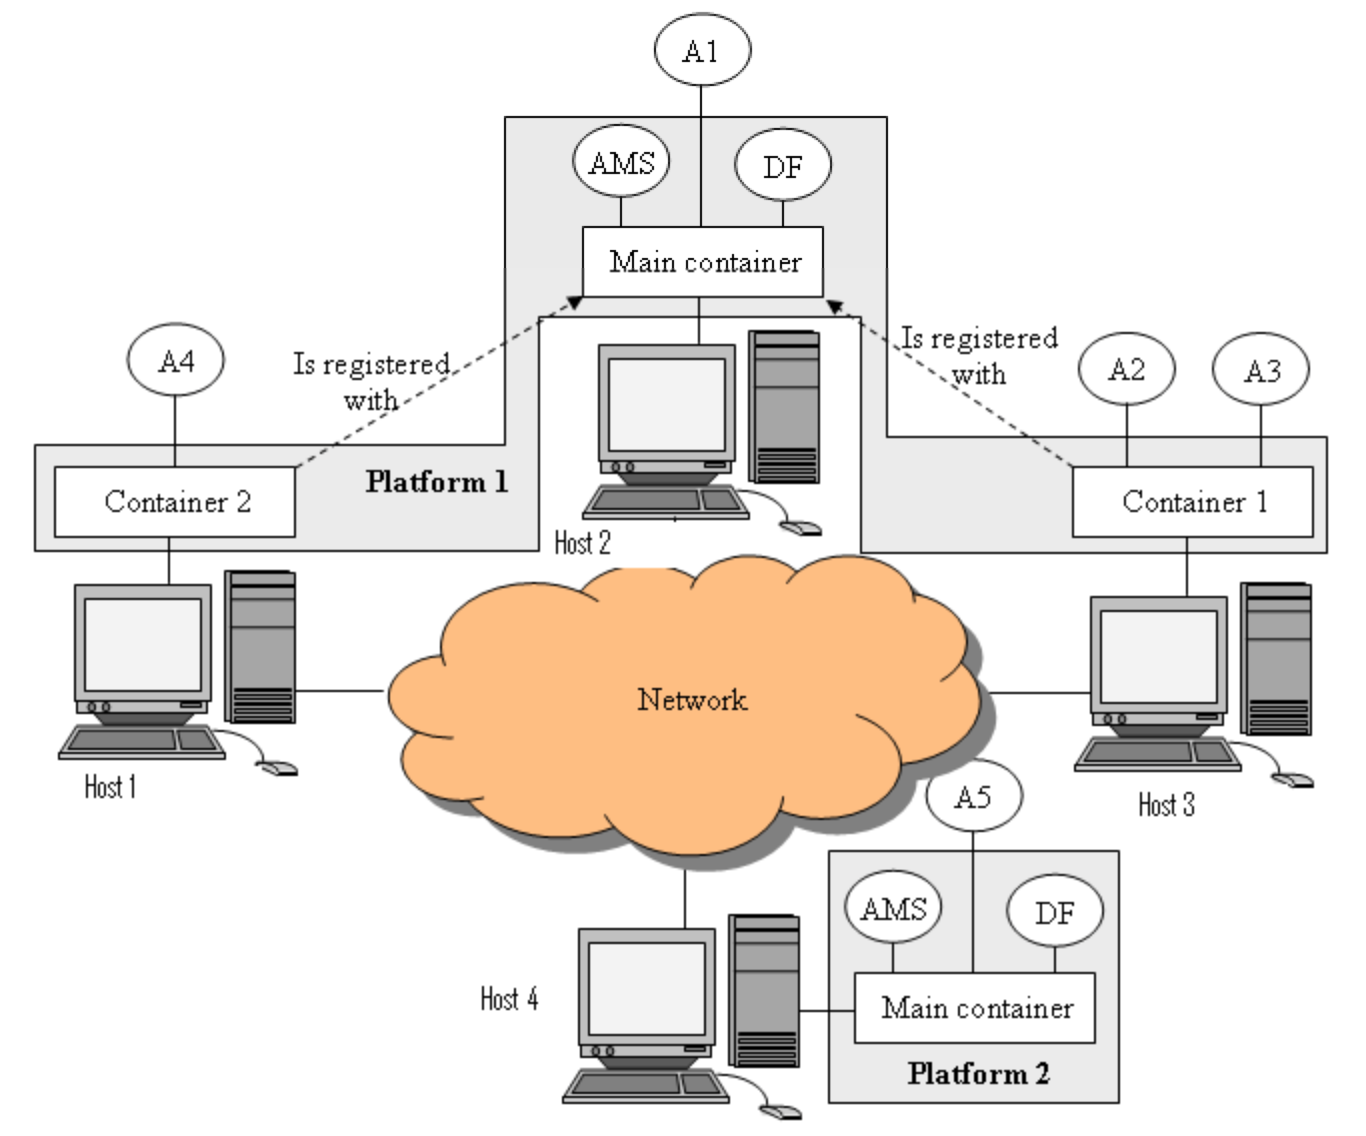
\includegraphics[width=10cm]{figuras/jade_architecture.png}
  \caption{Arquitetura do \textit{framework} JADE \cite{jadeArchitechture}}
  \label{figura:jade}
\end{figure}

\subsubsection{JADE para Android}

A plataforma JADE possui um conjunto de extensões que atendem a diversas
necessidades. Uma dessas extensões é o JADE para Android, uma extensão
necessária para que dispositivos Android possam implantar agentes JADE. Em
detalhes, o JADE é envolvido em um serviço específico Android. Um serviço
Android é um componente de aplicação que pode executar operações de longa
duração e que não fornecem uma interface para o usuário. Outros componentes da
aplicação podem iniciar um serviço e ele continuará a execução em
\textit{background} mesmo que o usuário mude de aplicação \cite{bergenti2014}.

O JADE para Android fornece uma interface que possibilita que aplicações
iniciem agentes, disparem comportamentos, e em geral, compartilhem dados entre
agentes. Por conseguinte, é possível descobrir pares remotos, realizar
conversas complexas, explorar ontologias JADE, executar atividades em
\textit{background} de acordo com o comportamento, e tirar proveito de todas as
funcionalidades do JADE \cite{bergenti2014}.

    \subsection{Plataforma WADE}

WADE (\textit{Workflows and Agents Development Environment}) \cite{wade},
versão 3.5.0, é a principal evolução do JADE. Ele adiciona a habilidade de
definir lógicas de sistema de acordo com a metáfora de fluxo de trabalho, além
de prover mecanismos que ajudam a gerir complexidades inerentes a Sistemas
MultiAgentes distribuídos. Tanto em administração, quanto em tolerância a
falhas \cite{wade2009}. Até o presente momento, o AMUSE utiliza o WADE apenas
pelas suas características de flexibilidade e escalabilidade em
\textit{deployment} \cite{bergenti2015}.

O principal componente da plataforma WADE é \textit{WorkflowEngineAgent}, uma
classe que estende o agente básico do JADE incorporando um pequeno e leve motor
de fluxo de trabalho. Além dos comportamentos normais do JADE, um
\textit{WorkflowEngineAgent} é capaz de executar fluxos de trabalho
representados de acordo com as especificações do WADE. Um fluxo de trabalho é
uma definição formal do processo em termos de atividades a serem executadas,
relações entre elas, critérios que especificam sua ativação e término, e
informações adicionais. As informações adicionais podem ser participantes,
ferramentas de software a serem invocadas, entradas requeridas, saídas esperadas
e informação manipulada durante a execução. Essa abordagem torna possível a
combinação da expressividade de metáforas de fluxo de trabalho com o poder de
uma linguagem de programação, como o Java; além de possibilitar o uso de fluxos
de trabalho para definição de lógicas internas de sistema \cite{wade}.

A Figura \ref{figura:wade} exemplifica a plataforma WADE. Os principais
componentes da plataforma são: JADE, responsável pelos agentes e comportamentos,
comunicação, e distribuição da execução; WADE, responsável pela construção do
fluxo de trabalho, administração e controle de falhas; \textit{Application}, a
aplicação desenvolvida com suas caracaterísticas específicas; WOLF
(\textit{WOrkflow LiFe cycle management environment}), ambiente de
desenvolvimento gráfico para a plataforma WADE, caso o usuário utilize a IDE
(\textit{Integrated Development Environment}) Eclipse.

\begin{figure}[h]
  \centering
  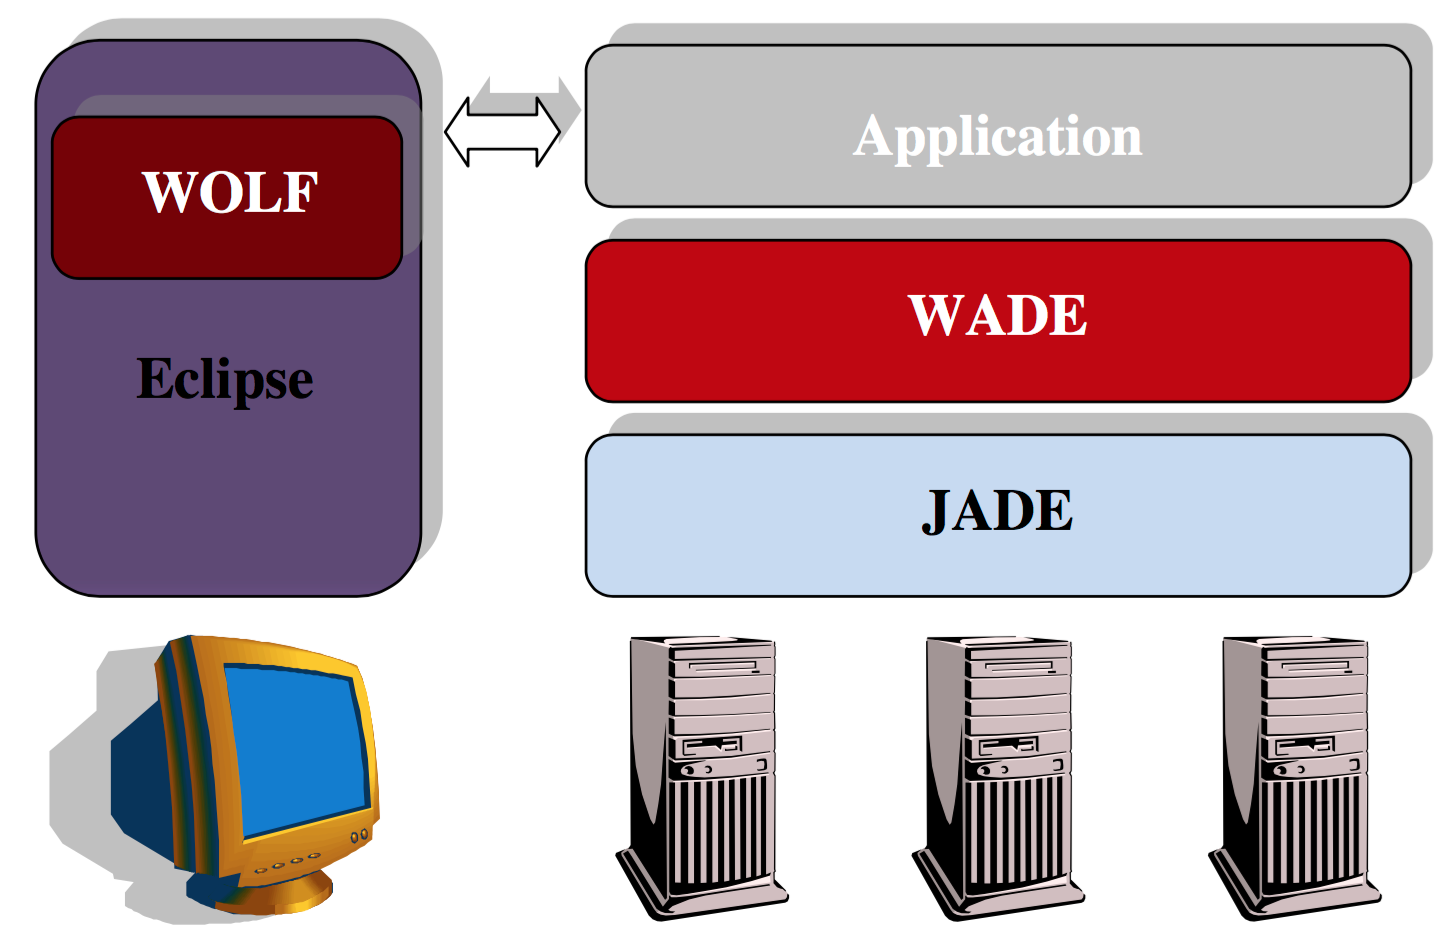
\includegraphics[width=10cm]{figuras/wade}
  \caption{Plataforma WADE \cite{wadeUserGuide}}
  \label{figura:wade}
\end{figure}

    \subsection{Plataforma AMUSE}

O AMUSE (\textit{Agent-based Multi-User Social Environment}) \cite{amuse},
versão 1.6.0, é uma plataforma de código aberto, baseada no JADE e WADE, que
facilita o desenvolvimento de aplicações sociais distribuídas que envolvem
usuários em atividades de cooperação e competição. O foco principal do AMUSE é
no suporte de jogos \textit{multi-player online} para o sistema Android. O
AMUSE utiliza a base do WADE e JADE para controlar todas as comunicações e
questões de gestão de componentes. A plataforma aborda aspectos relacionados à
organização, coordenação e sincronização de partidas entre jogadores. Ela não
oferece suporte para o desenvolvimento de interfaces gráficas.

\begin{figure}[h]
  \centering
  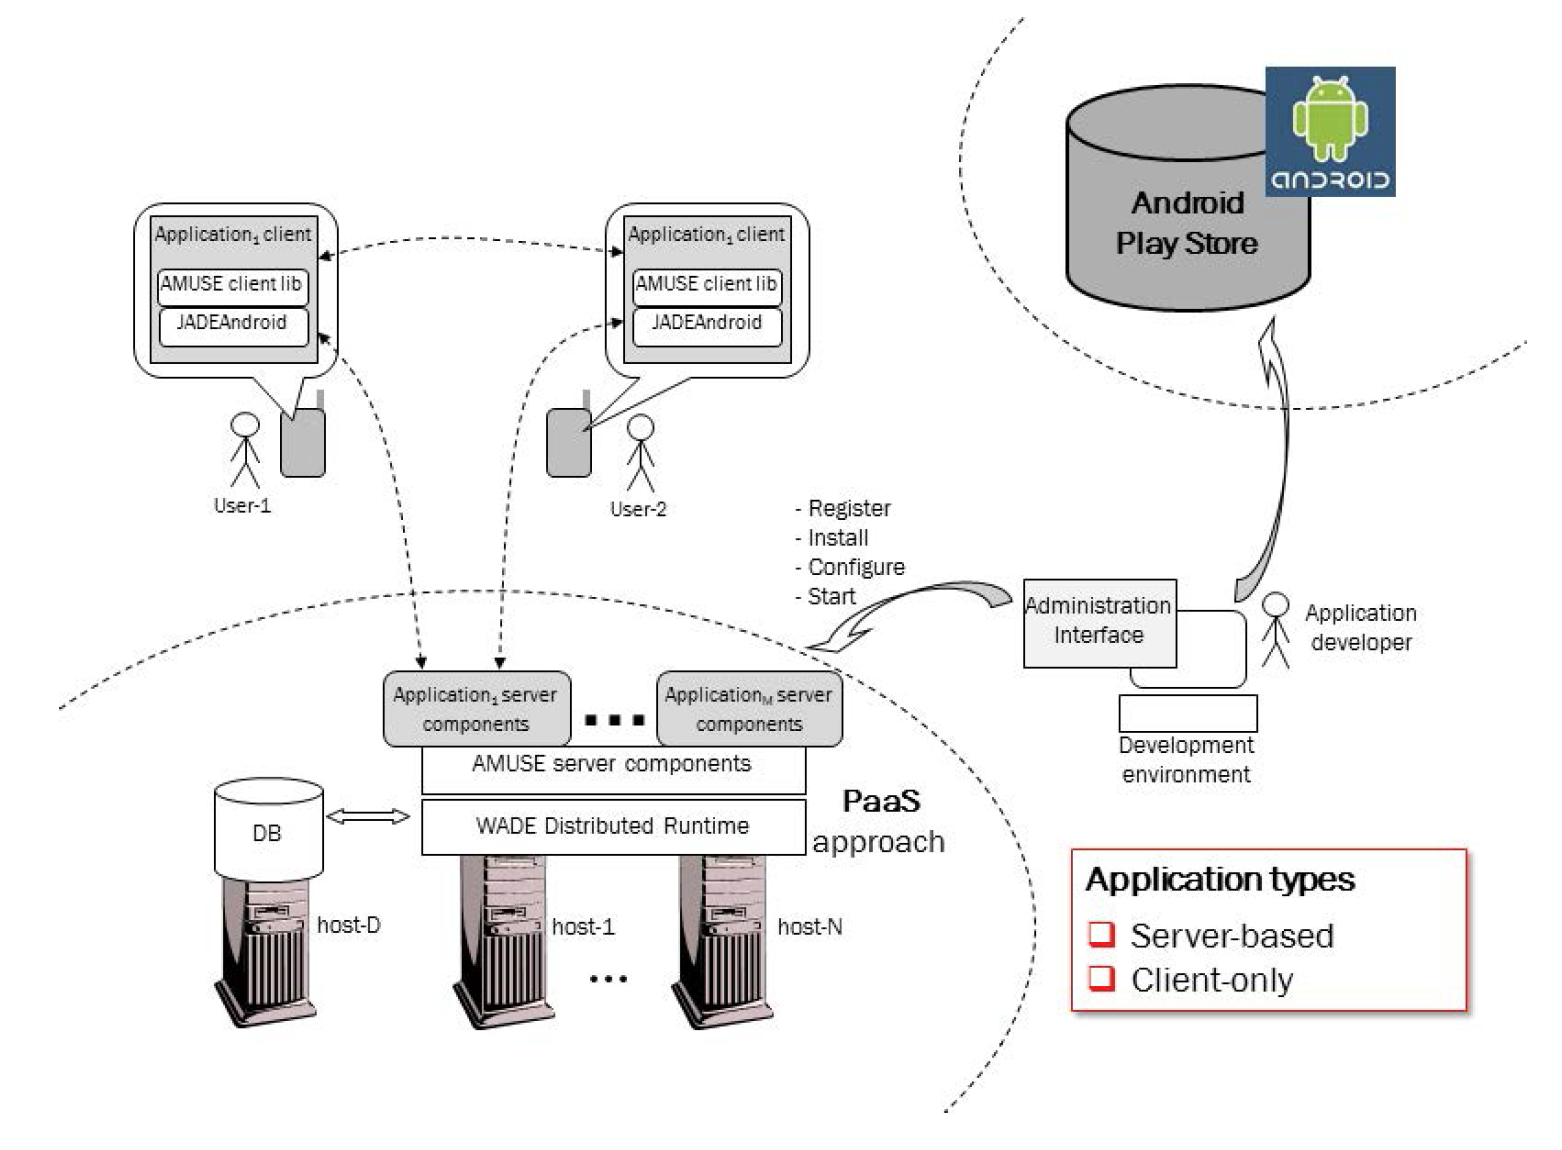
\includegraphics[width=13cm]{figuras/amuse_architecture}
  \caption{Visão arquitetural alto nível do AMUSE}
  \cite{bergenti2015}
  \label{figura:amuse_architecture}
\end{figure}

A Figura \ref{figura:amuse_architecture} mostra uma visão alto nível da
arquitetura do AMUSE. Todas as aplicações baseadas no AMUSE englobam um cliente
que fornece a interface com o usuário, e qualquer outra característica
específica de lógica do lado do cliente. A aplicação do lado do cliente faz uso
da biblioteca do AMUSE para interagir com outros usuários e com o servidor.
Aplicações que requerem execução de lógicas no lado do servidor contam com um
ambiente PaaS (\textit{Platform as a Service}) para essas execuções. Isso
significa que o AMUSE fornece componentes que tornam a plataforma prestadora de
serviço. A aplicação não tem conhecimento dos detalhes referentes a hardware,
sistemas operacionais e outras características do \textit{host}. Por outro
lado, eles são implementados em um ambiente de nuvem, e o AMUSE garante que a
aplicação tenha os recursos suficientes para sua execução
\cite{amuseStartupGuide}.

O AMUSE fornece um conjunto de funcionalidades que não estão estritamente
ligadas ao domínio de jogos. Essas funcionalidades são: \textit{Application
management}, \textit{User Management}, \textit{Clock synchronization},
\textit{Text message exchange}, \textit{Peer-to-peer pipe management} e
\textit{Centralized match coordination}. Essas funcionalidades são
implementadas através de recursos provenientes do JADE, WADE e agentes da
própria plataforma. Esse conjunto de agentes estão do lado do servidor, e do
lado do cliente. As interações entre esses diferentes tipos de agentes fornecem
a funcionalidade da plataforma. Os diferentes tipos de agentes disponibilizados
pela plataforma são \cite{bergenti2015}:

\begin{itemize}
  \item MMA\textit{(Match Manager Agent):} Este é o único agente no lado do usuário. Ele tem como responsabilidade fazer a interface entre o usuário e os agentes do lado do servidor, e executar tarefas que não necessitam de interação com os agentes do servidor;
  \item AMA\textit{(Application Manager Agent):} Agente responsável por realizar o controle dos jogos disponibilizados pela plataforma e seus ciclos de vida;
  \item GRA\textit{(Games Room Agent):} Agente responsável pelo controle dos dados compartilhados em jogos com interações síncronas;
  \item UMA\textit{(User Manager Agent):} Este agente realiza o controle dos perfis e relações dos usuários com os demais jogadores;
  \item MTA\textit{(Match Tracer Agent):} O agente MTA tem como objetivo suprir as necessidades dos jogos que necessitam de opções de reiniciar e persistir os seus estados.
\end{itemize}


\section{Ferramentas de Planejamento, Gerência e Desenvolvimento}
\label{sec:tecsuportedesenvolvimento}

Um conjunto de ferramentas foi selecionado para auxiliar o desenvolvimento
desse trabalho. Esse conjunto de ferramentas é necessário para a implementação
do código, teste, controle de versão e outras atividades inerentes ao escopo
desse projeto.

    \subsection{Teste de Software}
    \label{subsec:testedesoftwaresuptecnologico}

Para a realização de testes unitários, o \textit{framework} selecionado foi o
JUnit \cite{junit2015}, versão 4.12. JUnit é um \textit{framework} de código
aberto para escrita de testes repetíveis na linguagem Java. Ele é uma instância
da arquitetura xUnit para testes unitários.

Os testes de integração e de sistema são realizados com o suporte das
ferramentas disponibilizadas pela biblioteca ATSL \cite{atsl}. Essas
ferramentas são: Espresso, UI Automator e MonkeyRunner.

O Espresso \cite{espresso}, versão 2.2.2, é uma ferramenta para teste de
interface. Ele pode ser utilizado para testes caixa-preta. No entanto, o seu
potencial é totalmente aplicado quando implementado junto ao código do sistema.

O UI Automator \cite{uiAutomator}, versão 2.2.2, é uma ferramenta que torna
possível a realização de testes de integração entre vários aplicativos, e o
sistema Android.

O MonkeyRunner \cite{monkeyRunner}, versão 2.2.2, é uma ferramenta que permite
a criação de programas que controlam um dispositivo Android fora do contexto de
código Android. Através da criação desses programas, é possível implementar testes de integração e interface.

    \subsection{Controle de Versão}

Para o controle de versão do desenvolvimento do projeto, a ferramenta
selecionada foi o GIT \cite{git}. O Git é um sistema distribuído de controle de
versão, disponibilizado de maneira livre e código aberto. Ele é projetado para
lidar com projetos de diversos tamanhos com velocidade e eficiência. O
repositório do projeto está hospedado no GitHub \cite{gitHub}, que é um
repositório web baseado no Git. Ele oferece todas as funcionalidades de
controle de versão presentes no Git, como também adiciona suas próprias
funcionalidades.

    \subsection{Ferramentas de Desenvolvimento}
    \label{sec:tecferramentasdesenvolvimento}

As ferramentas de desenvolvimento selecionadas para o suporte ao projeto são:
Atom, LaTex, Eclipse, Android Studio e MacOS.

O Atom \cite{atom}, versão 1.16.0 x64, é um editor de texto de código aberto,
customizável, com suporte para todos os tipos de códigos abordados nesse
trabalho e disponível para os sistemas operacionais Mac OS, Windows e Linux.
Ele possui de forma nativa suporte para controle de versão através do Git.

LaTeX \cite{latex}, versão 2.7.5, é um sistema de preparação de documentos para
a composição tipográfica de alta qualidade. Ele inclui funcionalidades
projetadas para a produção técnica e científica de documentos.

O Eclipse \cite{eclipse}, versão Neon 3 (4.6.3), é uma IDE (\textit{Integrated
Development Environment}) \textit{open source} para desenvolvimento Java, com
suporte para outras linguagens através de plug-ins.

O Android Studio \cite{androidStudio}, versão 2.3.2 para MacOS, é uma IDE
(\textit{Integrated Development Environment}) para desenvolvimento de
aplicações Android, desenvolvida e distribuída pelo Google.

Por fim, o sistema operacional escolhido foi o Mac OS \cite{macos}, versão Mac
OS Sierra 10.12.5. Ele é desenvolvido pela Apple e baseado no Unix.

\section{Considerações Finais do Capítulo}

O objetivo desse capítulo foi descrever as ferramentas e tecnologias utilizadas
para apoio ao planejamento, gerenciamento e desenvolvimento do trabalho. A
seção \ref{sec:tecmultiagentes}, Sistemas MultiAgentes, descreveu as
tecnologias necessárias para a aplicação do paradigma MultiAgentes no contexto
de \textit{Mobile Social Games}. A seção \ref{sec:tecsuportedesenvolvimento},
Ferramentas de Planejamento, Gerência e Desenvolvimento, descreveu as
ferramentas necessárias para o suporte e desenvolvimento da proposta, aplicação
de boas práticas de Engenharia de Software, e escrita desse projeto.
